
\begin{figure}[h]
  \centering
  \begin{tabular}{  c p{0.7cm} c }
    \centering
    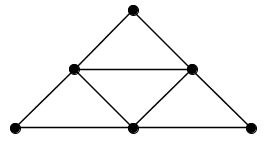
\includegraphics[width=4cm]{img/s3.png} & &
    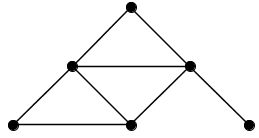
\includegraphics[width=4cm]{img/s3-1.png}
    \\
    \footnotesize \centering 
    (a)  \footnotesize Graph $S_3$ &&  \footnotesize (b) Graph $S_{3'}$ \\
    
    %---------------------
      \centering 
      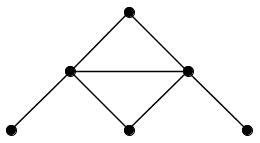
\includegraphics[width=4cm]{img/s3-2.png} & &
    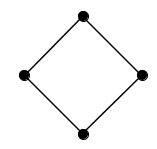
\includegraphics[width=3cm]{img/c4.png}
    \\
    \footnotesize \centering 
    (c)  \footnotesize Graph $S_{3''}$ && \footnotesize (b) Graph $C_{4}$\\
  \end{tabular}

 \caption{Set of subgraphs that define a  $B_1$-EPG-Helly subfamily}
 \label{fig:proibidos}
\end{figure} 
